\documentclass[11pt,a5paper]{article}

\usepackage[T1]{fontenc}
\usepackage[utf8]{inputenc}
\usepackage{lmodern, microtype}
\usepackage[estonian]{babel}
\usepackage{siunitx}
\sisetup{inter-unit-product=\ensuremath{{\cdot}}, per-mode=fraction, exponent-product=\cdot, output-decimal-marker={,}}
\usepackage{graphicx}
\usepackage{wrapfig}
\usepackage{adjustbox}
\usepackage{amsmath,amssymb}
\usepackage{amsfonts}
\usepackage[hidelinks]{hyperref}
\usepackage{csquotes}
\usepackage{caption}
\usepackage{enumitem}
\usepackage{soulutf8}
\topmargin=-3.0cm \textheight=19cm \textwidth=12.9cm
\oddsidemargin=-1.5cm  \evensidemargin=-1.5cm
\setlength{\parindent}{0pt} \setlength{\parskip}{6pt} \sloppy
\sloppy \relpenalty=10000 \binoppenalty=10000
\pagestyle{empty}

\newcommand{\numb}[1]{\vspace{5pt}\textbf{\large #1}}
\newcommand{\nimi}[1]{(\textsl{\small #1})}
\newcommand{\punktid}[1]{(\emph{#1~p.})}
\newcounter{ylesanne}
\newcounter{expylesanne}
\newcommand{\yl}[1]{\addtocounter{ylesanne}{1}\numb{\theylesanne.} \nimi{#1} \newblock{}}
\newcommand{\expyl}[1]{\addtocounter{expylesanne}{1}\numb{E\theexpylesanne.} \nimi{#1} \newblock{}}
\newcommand{\autor}[1]{}% Kasuta võistluse ajal
%\newcommand{\autor}[1]{\emph{Autor: #1}}% Kasuta kui vaja autorit

\begin{document}
\begin{center}
  \textbf{\Large Eesti koolinoorte 71. füüsikaolümpiaad} \par
  \emph{9. veebruar 2024. a. Piirkondlik voor.\\Gümnaasiumi ülesanded (10.--12. klass)}
\end{center}

\resizebox{\textwidth}{!}{
  \emph{%
    \begin{tabular}{@{}l@{}}
      \textbf{Palun kirjutada iga ülesande lahendus eraldi lehele.}\\
      Lahendamisaeg on 5 tundi. \\
      Iga osavõtja võib lahendada kõiki pakutud ülesandeid. \\
      Arvesse lähevad 5 suurima punktide arvu saanud teoreetilist ja 1 eksperimentaalne ülesanne. \\
      Kasutada võib kirjutus- ja joonestusvahendeid ning kalkulaatorit. Muud abivahendid on keelatud.\\
      Eksperimentaalülesande lahendamisel võib kasutada üksnes loetelus toodud vahendeid. \\
      Mõõtemääramatuse hindamist ei nõuta.
    \end{tabular}
  }
} \par


\yl{PÄIKESEPANEEL} Pille majapidamine tarbib aastas $\SI{3000}{\kWh}$ elektrit. Leidke, mitu päikesepaneeli on Pillel vähemalt vaja, et katta tema majapidamise energiakulu, kui iga päikesepaneeli pindala on $S = \SI{1.5}{\m\squared}$ ja kasutegur on $\eta = 15\%$. Eeldame, et Eestis on keskmine maapinnale langev päikeseenergia võimsus pindalaühiku kohta $I = \SI{110}{\W\per\m\squared}$ ning Pillel on piisavad võimalused energia salvestamiseks.
\punktid{6} \autor{Richard Luhtaru}

\yl{HAJUMINE} Juhanil on valgusallikas, mis tekitab paralleelset silindrikujulist valgusvihku, ning väike fotodetektorist tajur, mis mõõdab valguse intensiivsust. Esimeses katses mõõdab Juhan valgusallika intensiivsust, asetades tajuri täielikult valgusallika valgusvihku (ilma kumerpeeglita). Teises katses (vt joonis) suunab Juhan valgusvihu kumerpeeglile, mille kumerusraadius on $R=\SI{30}{\centi\m}$, nii et valgusvihk asub optilisel peateljel ja on sellega paralleelne. Seejärel mõõdab Juhan hajunud valguse intensiivsust, asetades tajuri täielikult peegeldunud valgusvihku (aga valgusallika enda valgusvihust kõrvale) peegli pinnast $L=\SI{60}{\centi\m}$ kaugusele. Mitu korda on tajuri näit esimeses katses suurem kui teises katses? Võib eeldada, et valgusallika valgusvihu laius on palju väiksem peegli kumerusraadiusest.
\punktid{6} \autor{Moorits Mihkel Muru}

\begin{figure}[h]
    \centering
    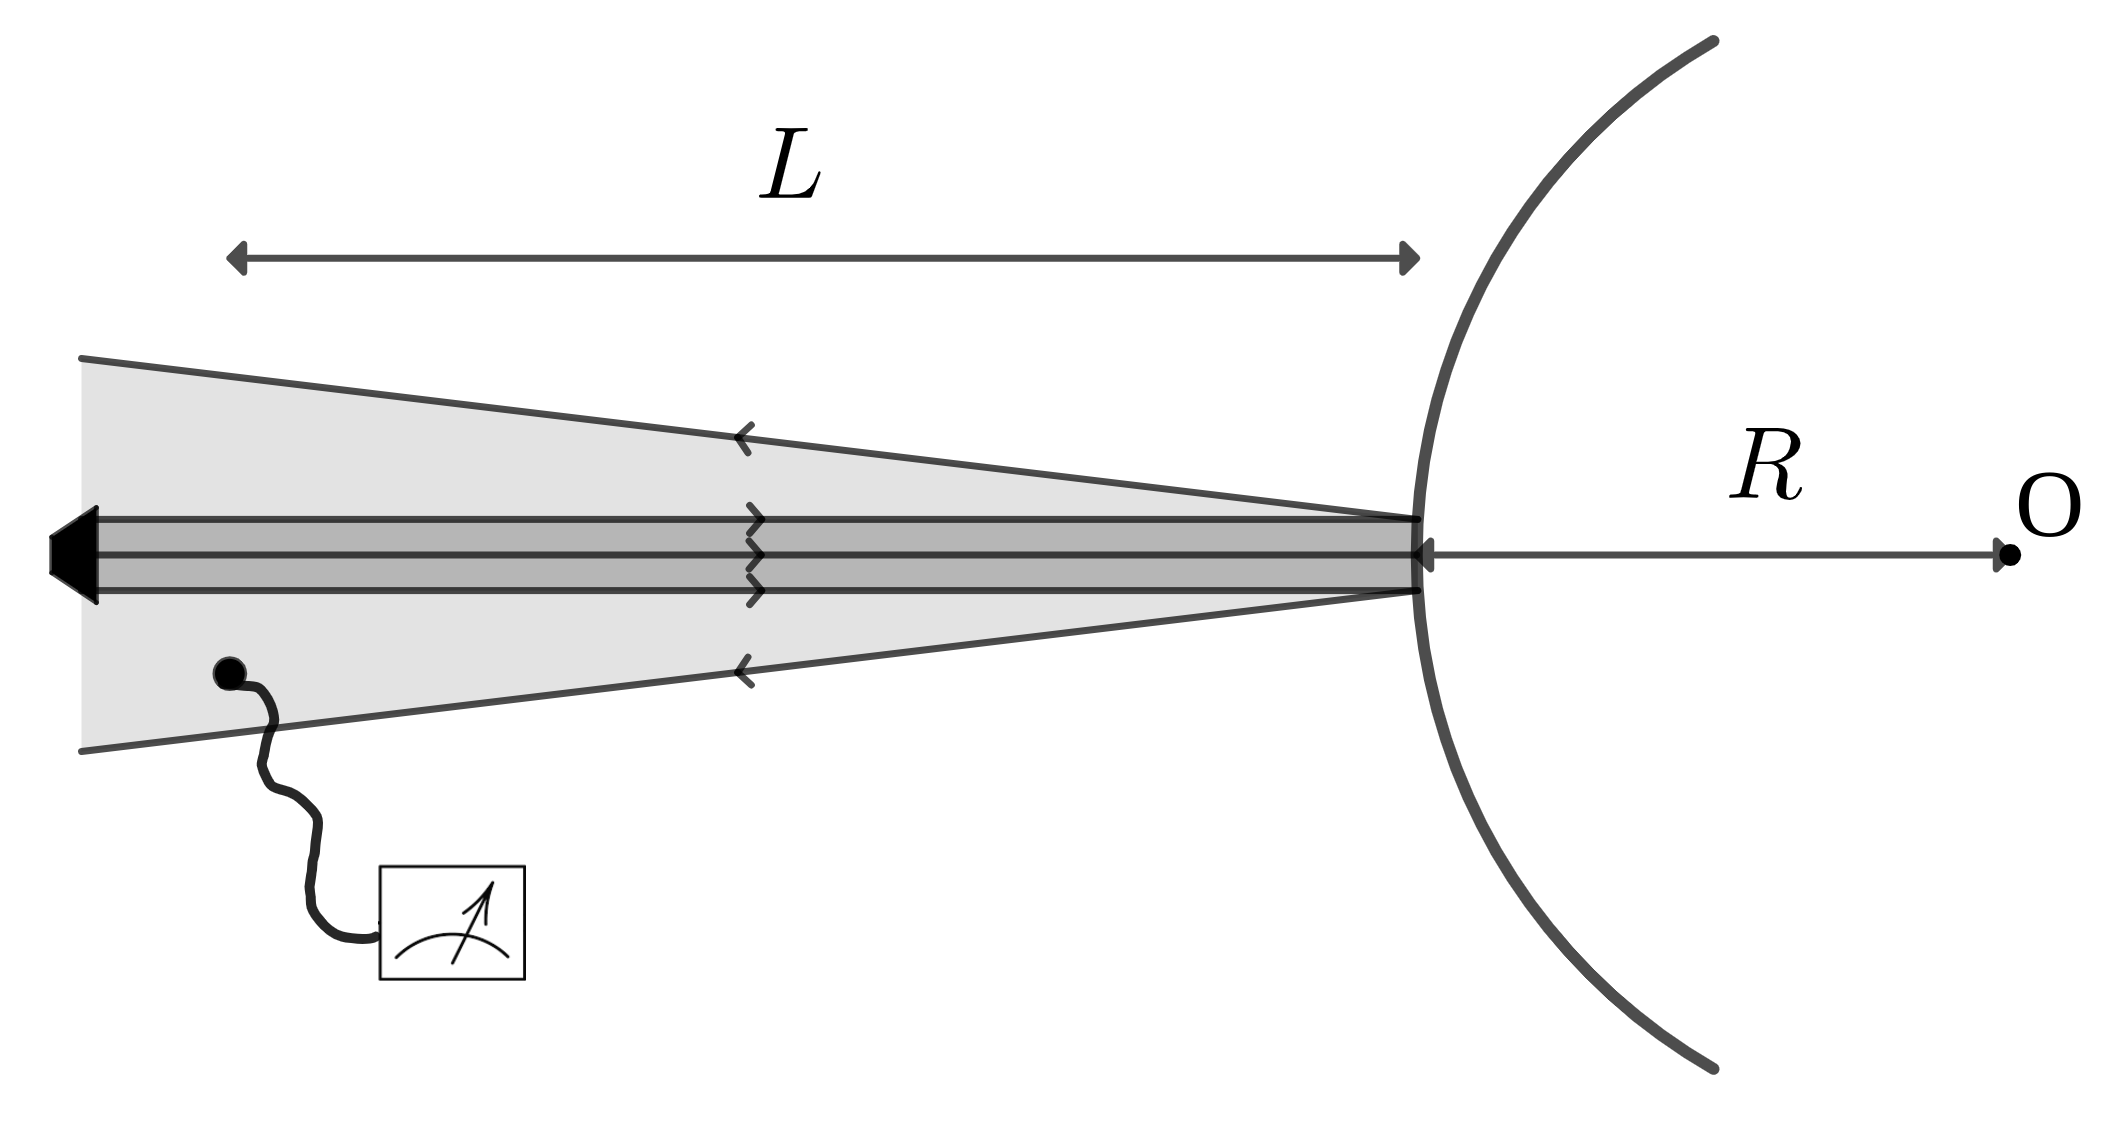
\includegraphics[width=0.6\linewidth]{hajumine-joonis-v3.png}
\end{figure}

\newpage

\begin{wrapfigure}{r}{0.5\textwidth}
  \vspace{-30pt}
  \begin{center}
  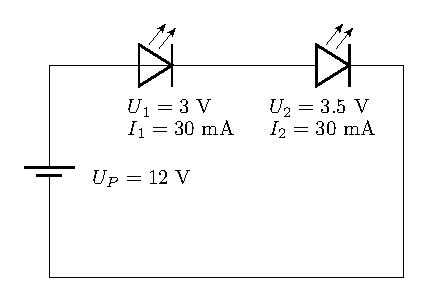
\includegraphics[scale=0.8]{Joonis_LEDid_yl.pdf}
  \vspace{-20pt}
  \end{center}
\end{wrapfigure}

\yl{VALGUSDIOODID} Mari koostas patareist ning kahest valgusdioodist (LEDist) vooluringi (vt joonist), kuid vooluahela kokkuühendamisel valgusdioodid põlesid läbi ning purunesid. Mari küsis isalt nõu, kes soovitas lisada vooluringi üks takisti. Aidake Maril välja mõelda, kui suure väärtusega takisti ja kuidas peaks ta skeemi lisama, et valgusdioodid töötaks normaaltingimustel. Joonistage uus vooluahel ning arvutage sobiva takisti väärtus. Patarei klemmipinge $U=\SI{12}{\V}$, valgusdioodide nimipinged on vastavalt $U_1=\SI{3}{V}$ ja $U_2=\SI{3.5}{V}$ ning optimaalne voolutugevus normaaltingimustel töötamisel $I_1=I_2=\SI{30}{\milli\A}$.
\punktid{8} \autor{Hans Daniel Kaimre}

\begin{wrapfigure}{r}{0.27\textwidth}
  \vspace{-25pt}
  \begin{center}
  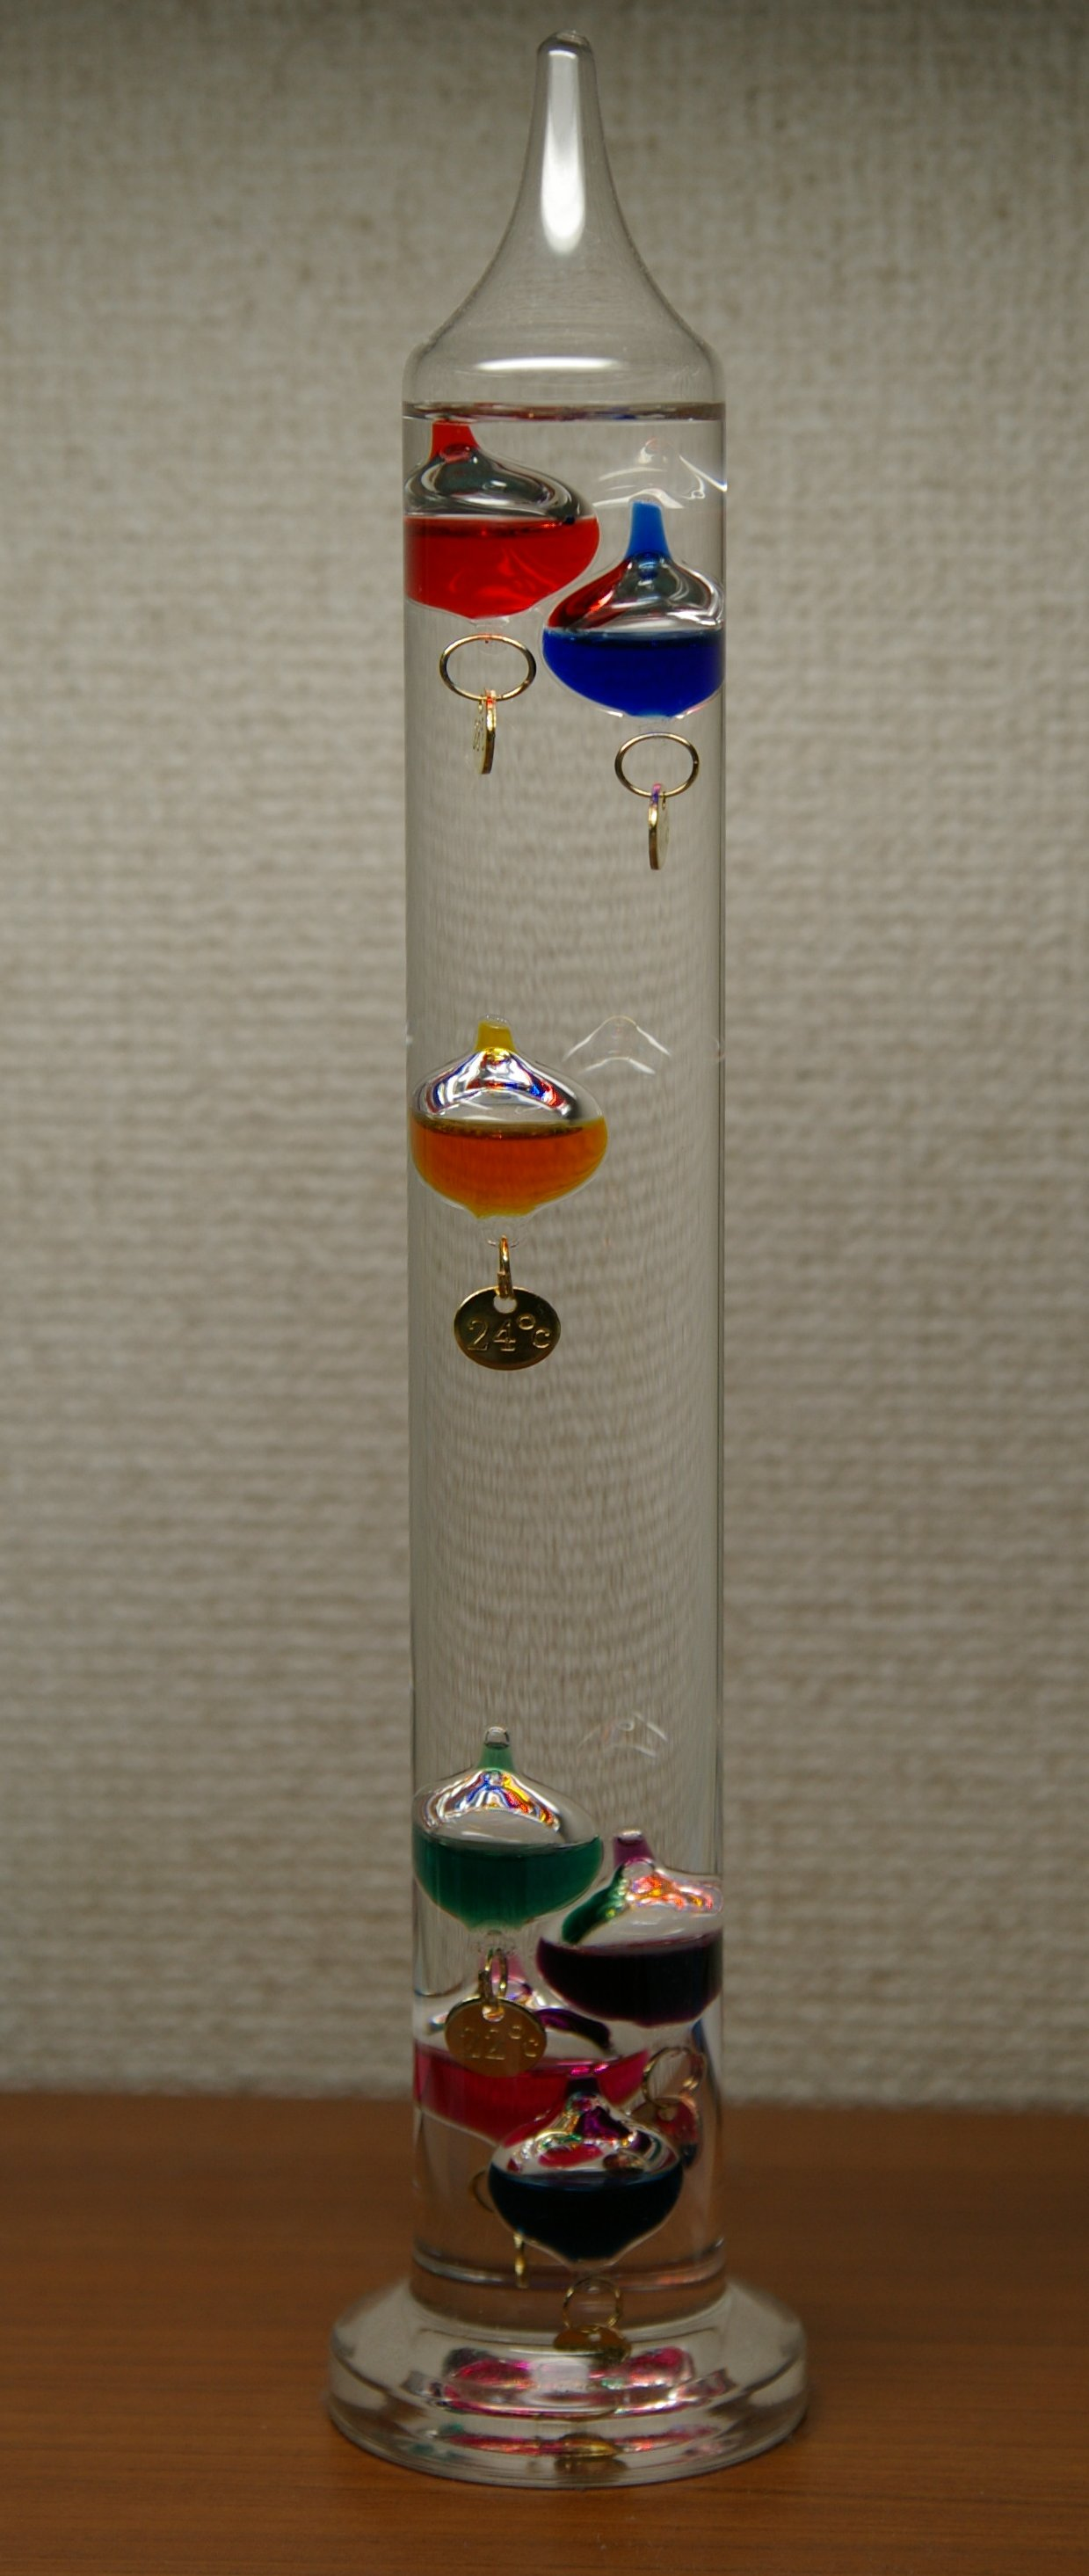
\includegraphics[scale=0.14]{GalileoT.jpg}
  \vspace{-20pt}
  \end{center}
\end{wrapfigure}

\yl{GALILEO TERMOMEETER} Galileo termomeetris (vt foto) hõljuvad vees erineva massiga, kuid sama ruumalaga kuulikesed (see ruumala arvestab nii kuulikest kui ka sinna külge kinnitatud sildikest). Kuulikeste keskmine tihedus on väga lähedane vee tihedusele. Et vee tihedus sõltub temperatuurist, siis sõltuvalt temperatuurist võib kuulike tõusta nii pinnale kui vajuda põhja. Kui teatud kuulike hõljub anuma põhja ja veepinna vahel, siis on temperatuur võrdne selle kuulikese külge kinnitatud sildil näidatud temperatuuriga. Silti $\SI{20}\celsius$ kandva kuulikese kogumass (koos sildikesega) on $m_1=\SI{20.000}{\g}$; milline on silti $\SI{22}\celsius$ kandva kuulikese mass? Vee ruumpaisumistegur on $k=\SI{2.1e-4}{\per\celsius}$, kuulikeste ruumpaisumistegur on sellest hulga väiksem. \textit{Vihje:} Ruumpaisumistegur kirjeldab ruumala suhtelist suurenemist temperatuuri tõusmisel $\SI{1}{\celsius}$ võrra, valemkujul: $\frac{\Delta V}{V} = k\Delta T$.
\punktid{8} \autor{Jaan Kalda}

\yl{AMOKSITSILLIIN} Juku läks tugeva kurguvaluga perearsti juurde, diagnoosiks osutus angiin ning Juku sai raviks $m= \SI{500}{\milli\gram}$ amoksitsilliinitabletid. Kui pika aja tagant on Jukul vaja üks tablett võtta? Juku kaalub $M= \SI{70}{\kilo\gram}$, ravimi minimaalne efektiivne kontsentratsioon kehakaalu kohta on $\SI{140}{\ug\per\kg}$. Amoksitsilliini poolestusaeg on $t= \SI{1.4}{\hour}$. \textit{Vihje:} Poolestusaja möödudes langeb aine kogus organismis poole võrra. Et ravim oleks efektiivne, peab selle kontsentratsioon kehas igal ajahetkel ületama minimaalset efektiivset kontsentratsiooni.
\punktid{8} \autor{Marten Rannut}

\begin{wrapfigure}{r}{0.33\textwidth}
\vspace{-20pt}
  \begin{center}
    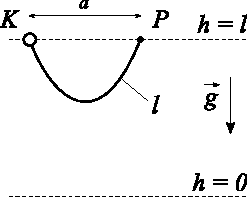
\includegraphics[width=1\linewidth]{me_noor_ajutine.pdf}
  \end{center}
  \vspace{-15pt}
\end{wrapfigure}

\yl{MITTEELASTNE NÖÖR} Väike kuulike on kinnitatud mitteelastse nööri külge ja seda hoitakse esialgu punktis $K$. Nööri pikkus on $l$ ja selle teine ots on kinnitatud punkti $P$. Punktid $K$ ja $P$ asuvad samal kõrgusel $h=l$ ja nendevaheline kaugus on $a$ ($0<a<l$). Nüüd lastakse kuulike ilma algkiiruseta vabaks ja see hakkab gravitatsiooni mõjul liikuma. Leidke maksimaalne kõrgus, mille kuulike saavutab $h=0$ suhtes edaspidise liikumise käigus (pärast täielikku kukkumist). Tehke kuuli trajektoori joonis. Nööri mass on võrreldes kuuli massiga tühine ning takistusjõududega võib mitte arvestada. Nööri mitteelastsus tähendab seda, et põrke hetkel summutab nöör kogu palli nöörisihilise impulsi.
\punktid{10} \autor{Päivo Simson}

\begin{wrapfigure}{r}{0.3\textwidth}
  \vspace{-25pt}
  \begin{center}
  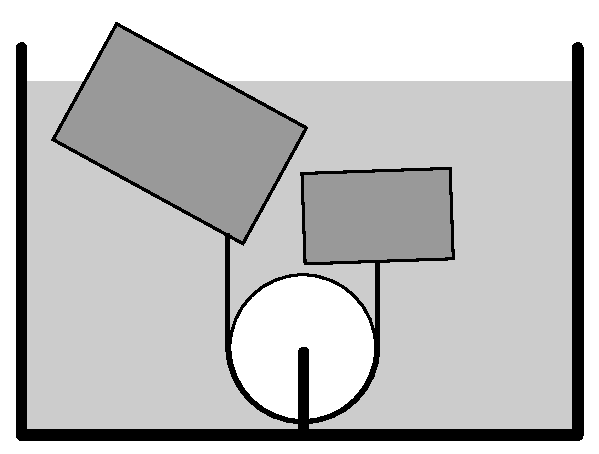
\includegraphics[scale=0.3]{palgid.pdf}
  \vspace{-20pt}
  \end{center}
\end{wrapfigure}

\yl{PALGID VEES} Kaks palki on kinnitatud üksteise külge nööri abil, mis läheb üle basseini põhja kinnitatud ploki nii nagu näidatud joonisel. Nöör on tõmmanud ühe palgi üleni vee alla sel ajal kui teine ujub vee pinnal. Mõlema palgi tihedus on $\rho=\SI {600}{\kg \per\m\cubed}$, vee tihedus $\rho_v=\SI{1000}{\kg\per\m\cubed}$, väiksema palgi ruumala on $V=\SI{30}\litre$ ja risttahuka kujulise basseini põhja pindala  $S=\SI{1}{m\squared}$. Kui palju muutub veetaseme kõrgus basseinis, kui palke ühendav nöör katki lõigata?
\punktid{10} \autor{Jaan Kalda}

\yl{HERMEETILINE SAUN} Aivo ehitas sauna $2\times 2\times 3$ meetri suuruse sauna, mille uks on $h=\SI{1.8}{\m}$ kõrge, $l=\SI{0.8}{\m}$ lai ning avaneb sissepoole. Aivo aga polnud väga kogenud ehitaja ja tegi sauna kogemata täielikult hermeetilise, nii et kinnise uksega puudub igasugune õhuvahetus sauna ja väliskeskkonna vahel. Ta pani saunaukse kinni, kui sauna temperatuur oli $T_1 = \SI{20}{\celsius}$, ja küttis seejärel sauna temperatuurini $T_2 = \SI{100}{\celsius}$. Kas Aivo saab nüüd ukse lükates lahti, kui ta kaalub $m=\SI{100}{\kg}$? Võib eeldada, et maksimaalne lükkejõud on piiratud Aivo ja põranda vahelise hõõrde poolt (hõõrdetegur $\mu=\num{0.6}$). Samuti võib eeldada, et väljas on ühtlaselt rõhk $p_0=\SI{101 000}{\Pa}$, sauna soojenemisel kehtib ideaalgaasi võrrand ja ukselink asub ukse servas.
\punktid{12} \autor{Hannes Kuslap}

\begin{wrapfigure}{r}{0.3\textwidth}
  \vspace{-25pt}
  \begin{center}
  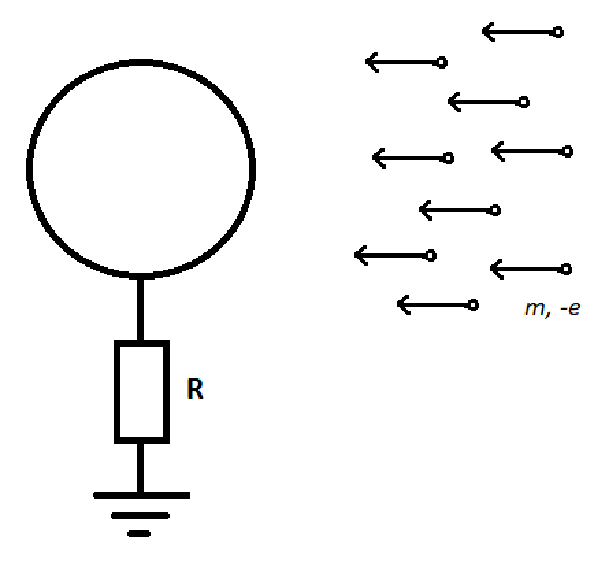
\includegraphics[width=\linewidth]{laetud-kuul-joonis-v2.png}
  \vspace{-30pt}
  \end{center}
\end{wrapfigure}

\newpage

\yl{LAETUD KUUL} Metallist kuul raadiusega $a$ on maandatud takistuse $R$ kaudu, vt joonist. Kuulile on suunatud lai elektronide (mass $m$, laeng $-e$) voog, kus elektronide kiirus on $v$ ja elektronide arv ruumalaühiku kohta on  $n$. Millise laengu omandab kuul tasakaalulise olukorra saabudes? Elektronide kiirus on nii suur, $v \gg n e^2 a^2 R / m$, et kuulile kogunev laeng ei suuda nende trajektoori märkimisväärselt kõverdada. Arvtihedus $n$ on nii väike, et elektronide tekitatud elektriväljaga võib mitte arvestada. \textit{Vihje:} Kui kuul kannab laengut $Q$, siis tema pinge maapinna suhtes on $\varphi = \frac{Q}{4\pi\varepsilon_0 a}$.
\punktid{12} \autor{Konstantin Dukatš}

\begin{wrapfigure}{r}{0.25\textwidth}
\vspace{-25pt}
  \begin{center}
    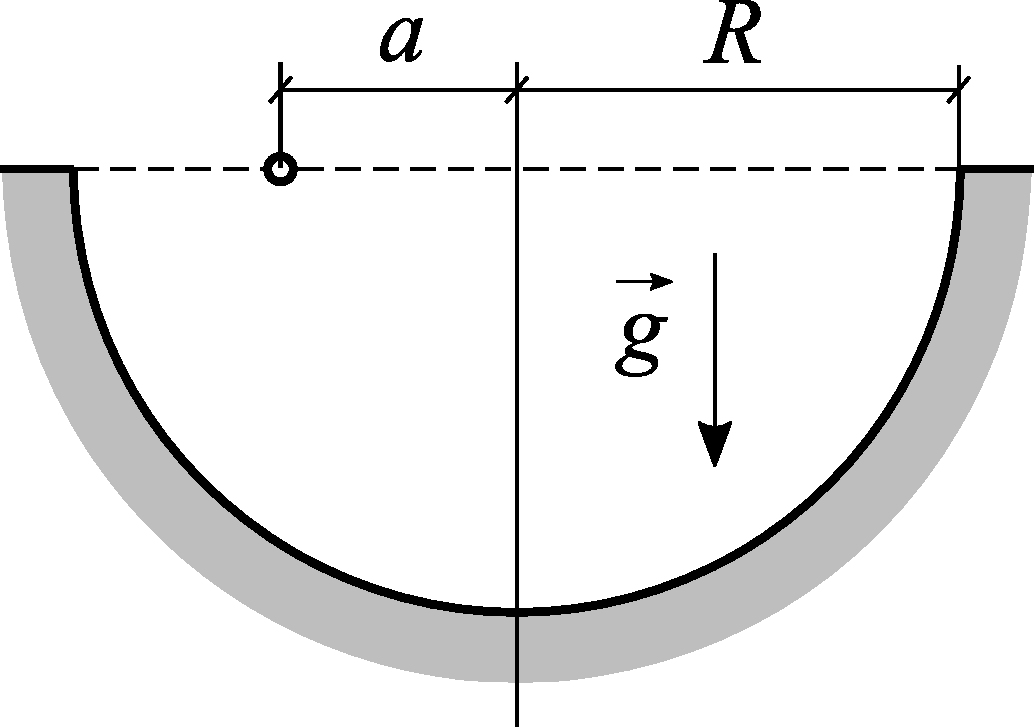
\includegraphics[width=\linewidth]{porked_fig.pdf}
    %\caption{}
  \end{center}
  \vspace{-1cm}
\end{wrapfigure}

\yl{PÕRKED} Väiksel kummipallil lastakse kukkuda poolkera sisse, mille raadius on $R$. Kõrvaloleval lõikel on näidatud palli algne asukoht, mis on kaugusel $a$ kera tsentrist. Palli algkiirus on null. Leidke üks selline kaugus $a$ ($0<a<R$), mille korral liikumine pärast esimest põrget on perioodiline.
\punktid{14} \autor{Päivo Simson}

\end{document}